% CVPR 2022 Paper Template
% based on the CVPR template provided by Ming-Ming Cheng (https://github.com/MCG-NKU/CVPR_Template)
% modified and extended by Stefan Roth (stefan.roth@NOSPAMtu-darmstadt.de)

\documentclass[10pt,twocolumn,letterpaper]{article}

%%%%%%%%% PAPER TYPE  - PLEASE UPDATE FOR FINAL VERSION
%\usepackage[review]{cvpr}      % To produce the REVIEW version
\usepackage{cvpr}              % To produce the CAMERA-READY version
%\usepackage[pagenumbers]{cvpr} % To force page numbers, e.g. for an arXiv version

% Include other packages here, before hyperref.
\usepackage{graphicx}
\usepackage{amsmath}
\usepackage{amssymb}
\usepackage{booktabs}
\usepackage{hyperref}
\usepackage{subcaption,graphicx}
\usepackage{lipsum}
\hypersetup{
    colorlinks=true,
    linkcolor=blue,
    filecolor=magenta,      
    urlcolor=cyan,
    pdftitle={Overleaf Example},
    pdfpagemode=FullScreen,
    }
    
\urlstyle{same}


% It is strongly recommended to use hyperref, especially for the review version.
% hyperref with option pagebackref eases the reviewers' job.
% Please disable hyperref *only* if you encounter grave issues, e.g. with the
% file validation for the camera-ready version.
%
% If you comment hyperref and then uncomment it, you should delete
% ReviewTempalte.aux before re-running LaTeX.
% (Or just hit 'q' on the first LaTeX run, let it finish, and you
%  should be clear).
\usepackage[pagebackref,breaklinks,colorlinks]{hyperref}

\usepackage{caption}
% Support for easy cross-referencing
\usepackage[capitalize]{cleveref}
\crefname{section}{Sec.}{Secs.}
\Crefname{section}{Section}{Sections}
\Crefname{table}{Table}{Tables}
\crefname{table}{Tab.}{Tabs.}


%%%%%%%%% PAPER ID  - PLEASE UPDATE
\def\cvprPaperID{*****} % *** Enter the CVPR Paper ID here
\def\confName{CVPR}
\def\confYear{2022}


\begin{document}

%%%%%%%%% TITLE - PLEASE UPDATE
\title{Team 4 - Midterm Project Report}

\author{Tadipatri Uday Kiran Reddy\\
{\tt\small ee19btech11038@iith.ac.in}
% For a paper whose authors are all at the same institution,
% omit the following lines up until the closing ``}''.
% Additional authors and addresses can be added with ``\and'',
% just like the second author.
% To save space, use either the email address or home page, not both
\and
Sahukari Chaitanya Varun\\
{\tt\small ee19btech11040@iith.ac.in}
\and
L. Pranay Kumar Reddy\\
{\tt\small ai19btech11019@iith.ac.in}
}
\maketitle

%%%%%%%%% ABSTRACT
\begin{abstract}
With the evolution of high-resolution digital cameras, snapshots have become the most common way to record and share visual data and experiences taken through mobile phones and tablets. But as humans, it is challenging to keep a stiff hold while capturing an image, especially when the image is to be captured on the move; it introduces blur. Though there lot of external tools for frame stabilization, such as gimbal, mounting it on can be challenging at times. Hence, we propose this paper to solve this problem by processing the image with the aid of gyroscope sensed data  attached with the camera device, helping to deblur the image. We aim to implement this deblurring with the help of deep convolution nets and extrapolate it with GAN's to give better quality and faster output than  traditional CNN's. We can extend this work to stabilise the video feed with lower frame rates with faster computation capabilities.
\end{abstract}

%%%%%%%%% BODY TEXT

\label{sec:intro}
% Introduce the problem you are working on. This section should give a general introduction motivation for the problem. You can also describe the applications of your problem here. 

% Please number all of your sections and displayed equations as in these examples:
% \begin{equation}
%   E = m\cdot c^2
%   \label{eq:important}
% \end{equation}
% and
% \begin{equation}
%   v = a\cdot t.
%   \label{eq:also-important}
% \end{equation}
%-------------------------------------------------------------------------
\section{Further literature review}
With the ever-growing classical image processing problem, deblurring is also a key research area that has witnessed significant progress. There are major three types of deblurring; Burst mode assisted deblurring, non-blind deblurring and blind deblurring(also known as single image-based deblurring);  Burst-mode assisted deblurring, also known as deblurring using multiple images, as it describes series of images are captured for a scene and using these the deblurred images are estimated recent works like \cite{article}, \cite{10.1145/1141911.1141956} focused on statistics approach to estimate blur-kernels or Point Spread Function (PSF) and applying deconvolution on the image to get the latent image. Authors of \cite{Aittala_2018_ECCV} use the Convolutional Neural Network(CNN) approach to deblur the image; here, the PSF approach is not adopted. In non-blind deblurring, blur-kernel or PSF available priorly these works \cite{8578443}, \cite{6618928} render perfect images but this method is not practically feasible as the PSF is not priorly known always. In blind deblurring, alone single image is exploited to deblur the image, classically blur-kernel is estimated later a  deconvolution operation is applied on the image to get the latent image. Authors of \cite{8237771}, \cite{6126276} use a statistical approach to estimate the PSF, albeit they assume that blur is space-invariant. In simpler words, they assume the blur is linear throughout the image, albeit images experience non-linear blur. Intuitively, we see that estimating the blur kernel followed by deconvolution is not flawless and adds artefacts that may render an undesirable latent image. Smartphones or DSLR cameras are equipped with sensors like gyroscopes, accelerometers and magnetometers. Recent works \cite{7780574}, \cite{Sindelar2013ImageDI}, \cite{9444479}, \cite{8820138}, \cite{mustaniemi2018gyroscopeaided} exploit such data to deblur the images but works \cite{Sindelar2013ImageDI}, \cite{9444479}, \cite{8820138}, \cite{mustaniemi2018gyroscopeaided} take an impractical assumption that blue is space-invariant and also assume that sensor data is reliable. But these are prone to time delay, miscalibration and anomalies. Authors in \cite{mustaniemi2018gyroscopeaided} showed incredible results despite these assumptions; here, they built their architecture based on Encoder-Decoder CNN with a pre-computed 2-channel blur field. In \cite{7780574}, the authors have considered the sensor’s non-idealities. The authors also compute the blur-field with sensor data but also refine it by solving an optimisation problem. 
\section{Deep Gyro \cite{mustaniemi2018gyroscopeaided} Implementation}
This section covers on the \href{https://drive.google.com/drive/folders/1Lh97DlusYyZEkIuu9gvTZXaLcDK3dlXc?usp=sharing}{implementation} of deblurring of images using gyroscope-extracted data with help a deep neural network. This deblurring is based fully-convolutional neural network. For working on this problem in a supervised manner we need data.
\subsection{Data for Playing}
For training the network, we need a set of blurred and sharp images along with the corresponding gyro-based blur fields. But manually capturing this data data in real time is difficult. So we use gyroscope readings to generate realistic blur fields and blurred images. For this purpose, the visual-inertial dataset has been used which is a set diverse sequences in different scenes for evaluating odometry. IMU measurements in the dataset has the measurements of accelerations and angular velocities on 3 axes at 200 Hz. We extract the gyro data for generating the blur fields. Here, two different blur fields are generated referred to as "exact" and "noisy" , where the exact blur field is used in generating the blurred image and the noisy blur field is given to network as additional input to help in deblurring. 
\begin{figure*}[h]
    \centering
    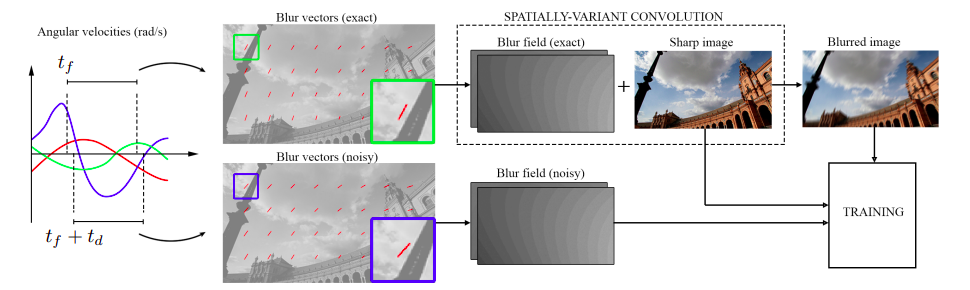
\includegraphics[width=2.2\columnwidth,height=6cm]{images/dat_gen.png}
    \caption{ Data generation schematic picture}
    \label{fig: data_generation}
\end{figure*}
\begin{figure*}[h]
    \centering
    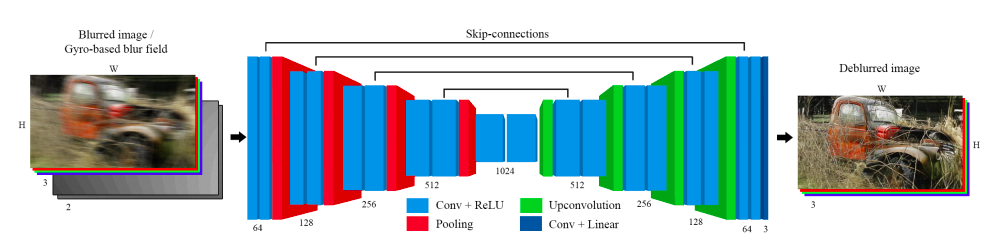
\includegraphics[width=2.2\columnwidth,height=5cm]{images/architecture.png}
    \caption{ Network Architecture}
    % \source{Gyroscope-Aided Motion Deblurring with Deep Networks}
    \label{fig: result_deepgyro}
\end{figure*}\\
The calibration parameters  of the camera device which include camera intrinsics, camera readout time, IMU-camera temporal offsets, IMU-to-camera rotation is taken into consideration so that if we downsample the picture, the camera intrinsics also have to be scaled accordingly and help in computation of blur field. Along with them, the time stamps and exposure times data is also used for computing the blur field. For the purpose of further training of our model, we try to inculcate the DAVIS 240C dataset for pose estimation, visual odometry and SLAM. 
\subsection{Generating Blur Fields}
As described in PPR, the same approach is taken for the blur estimation. To make the model more robust, the exposure times and read out times are slightly but randomly tweaked to simulate the misalignment between the camera and the gyroscope. A small uniformly random delay is added when computing the noisy blur field. We first rotate the gyroscope measurements from IMU frame to the camera frame. The gyroscope reading are then upsampled to facilitating readings for the time difference between two consecutive row exposures. The rotation of camera is estimated by integrating the gyroscope readings and futher fid the quaternions to rotation matrices. Then the blur fields are computed based on the horizontal and vertical components of the blur by finding the projections as discussed in the PPR. These blur vectors are returned as a gray scale image for the neural network.

\begin{figure}
\centering
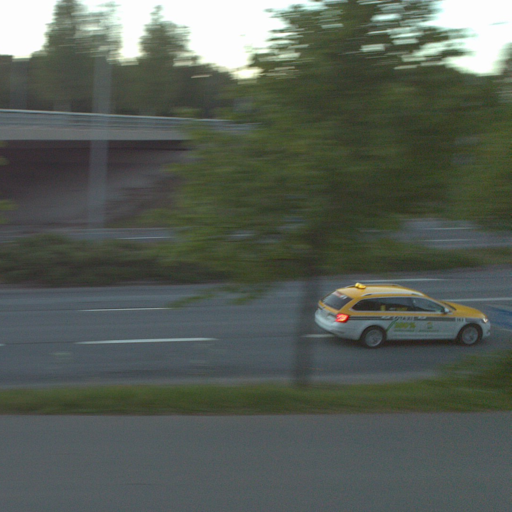
\includegraphics[width=.3\textwidth]{images/car.png}\hfill
\subcaption{Blurred Image}

\includegraphics[width=.3\textwidth]{images/car_x.png}\hfill
\subcaption{Blur Field X-component}

\includegraphics[width=.3\textwidth]{images/car_y.png}
\subcaption{Blur Field Y-component}
\caption{Example for generation of blur field}
\label{fig:figure3}
\end{figure}
\subsection{Network Architecture}
This network architecture is similar to that of encoder-decoder network which is generally used in image translation problems. The input of the network consists of blurred RGB image and a gyro-based blur field. They pass through series of convolutional and downsampling layers, until the lowest resolution is reached and then after the bottlenecke, the low resolution image is expanded to full resolution image with the help of upsampling layers and skip connections, which helps in information exchange between the encoder and decoder network.
%\begin{figure*}[h]
%    \centering
%    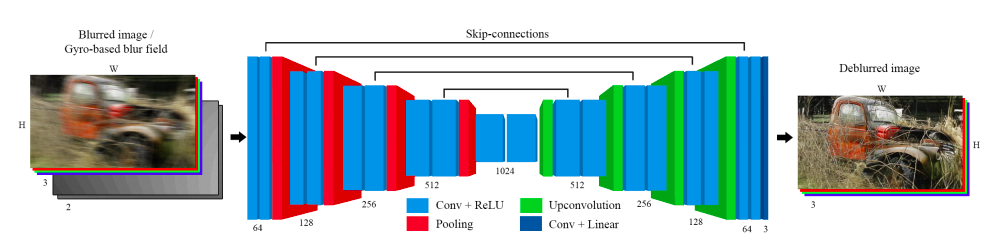
\includegraphics[width=2.2\columnwidth,height=5cm]{images/architecture.png}
%    \caption{ Network Architecture}
%    % \source{Gyroscope-Aided Motion Deblurring with Deep Networks}
%    \label{fig: result_deepgyro}
%\end{figure*}
As shown the network has 5 convolution layers for downsampling and 5 for upsampling. The output of each convolution layer is padded accordingly.The stride is 2 in 2$\times$ 2 max pooling in downsampling and the upconcolution layers have 2$\times$2 convolution that halves the number of feature channels. 

\subsection{Training and Results}

The model uses Adam optimizer for fitting the data. ReLu-activation used for all layers except the last layer which has linear activation. Original model was trained on 100k images, we used the weights of the pre-trained model to test for the initial phase.The results are as shown in Figure \ref{fig:ExampleBlurField}

\begin{figure}[h]
  \centering
  \begin{subfigure}{.5\columnwidth}
    \centering
    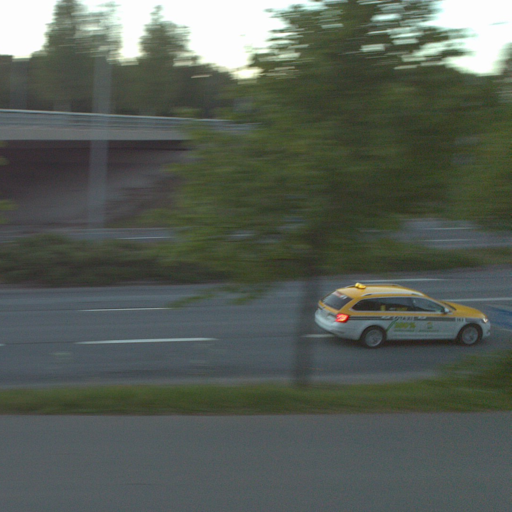
\includegraphics[width=\linewidth]{images/car.png}
  \end{subfigure}%
  \hfill
  \begin{subfigure}{.5\columnwidth}
    \centering
    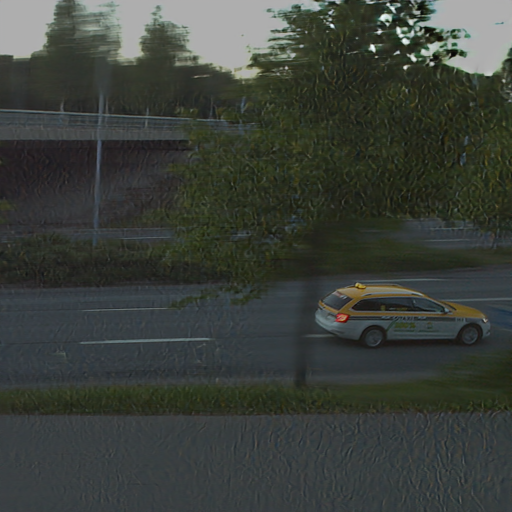
\includegraphics[width=\linewidth]{images/car_dg.png}
  \end{subfigure}%
  \hfill
\end{figure}
\vspace{-1cm}
\begin{figure}[h]
  \centering
  \begin{subfigure}{.5\columnwidth}
    \centering
    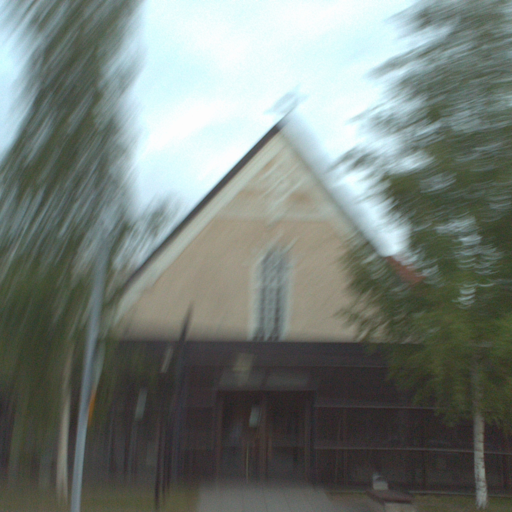
\includegraphics[width=\linewidth]{images/church.png}
  \end{subfigure}%
  \hfill
  \begin{subfigure}{.5\columnwidth}
    \centering
    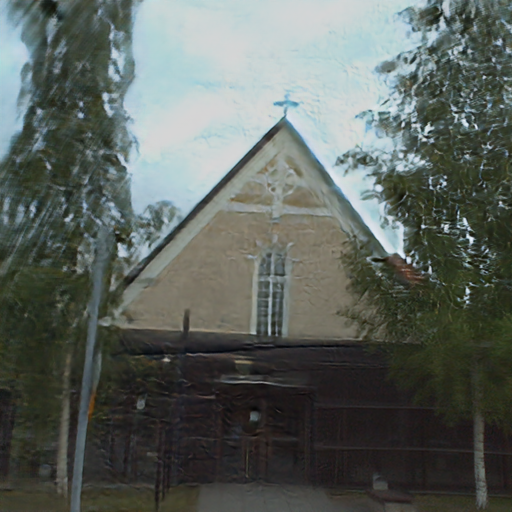
\includegraphics[width=\linewidth]{images/church_dg.png}
  \end{subfigure}%
  \hfill
\end{figure}
\vspace{-1cm}
\begin{figure}[h]
  \centering
  \begin{subfigure}{.5\columnwidth}
    \centering
    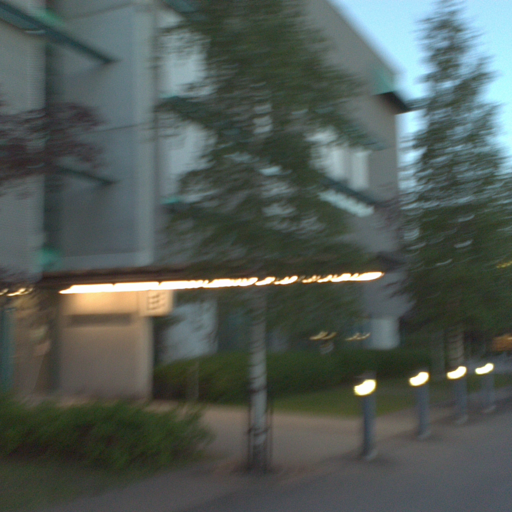
\includegraphics[width=\linewidth]{images/entrance.png}
  \end{subfigure}%
  \hfill
  \begin{subfigure}{.5\columnwidth}
    \centering
    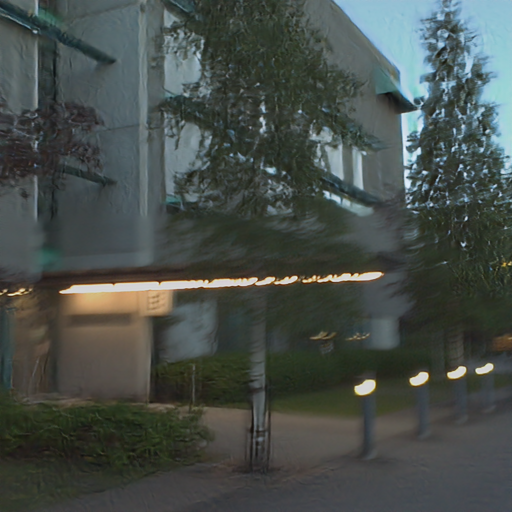
\includegraphics[width=\linewidth]{images/entrance_dg.png}
  \end{subfigure}%
  \hfill
\end{figure}
\vspace{-1cm}
\begin{figure}[h]
  \centering
  \begin{subfigure}{.5\columnwidth}
    \centering
    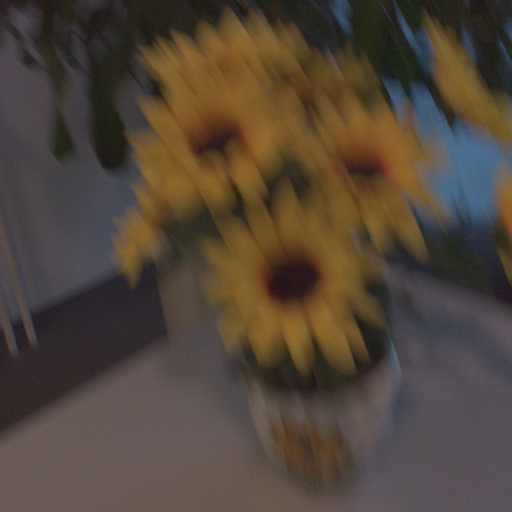
\includegraphics[width=\linewidth]{images/flower.png}
  \end{subfigure}%
  \hfill
  \begin{subfigure}{.5\columnwidth}
    \centering
    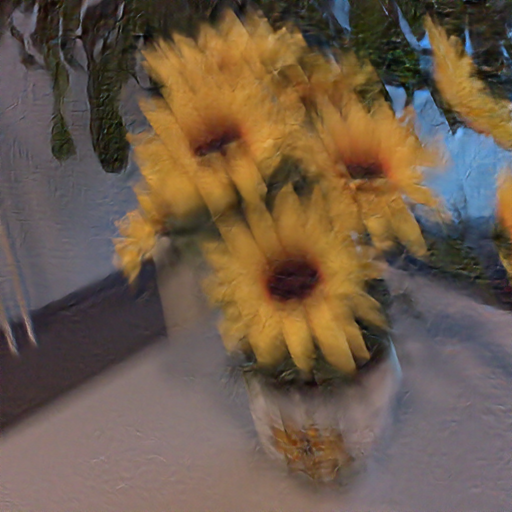
\includegraphics[width=\linewidth]{images/flower_dg.png}
  \end{subfigure}%
  \hfill
  \caption{Results replicated from the paper(blurred on left, deblurred on right)}
  \label{fig:ExampleBlurField}
\end{figure}
% \vspace{-1cm}
% \begin{figure}[h]
%   \centering
%   \begin{subfigure}{.5\columnwidth}
%     \centering
%     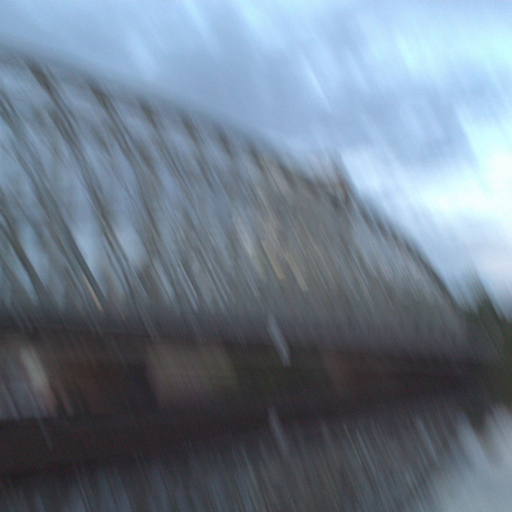
\includegraphics[width=\linewidth]{images/bridge.png}
%   \end{subfigure}%
%   \hfill
%   \begin{subfigure}{.5\columnwidth}
%     \centering
%     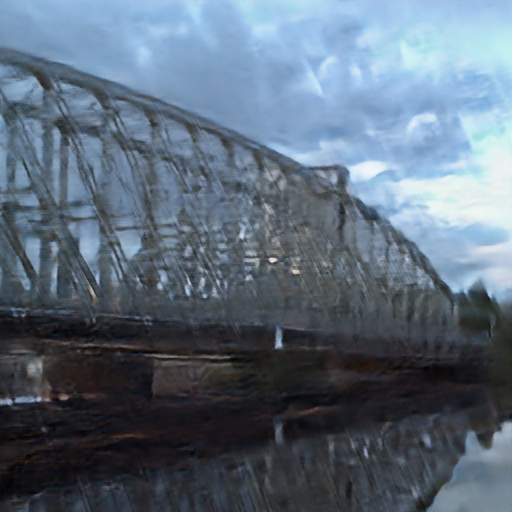
\includegraphics[width=\linewidth]{images/bridge_dg.png}
%   \end{subfigure}%
%   \hfill
%   \caption{Results replicated from the paper(blurred on left, deblurred on right)}
%   \label{fig : ExampleBlurField}
% \end{figure}


% \begin{figure}[h]
%     \centering
%     \subfloat[Blurred]{{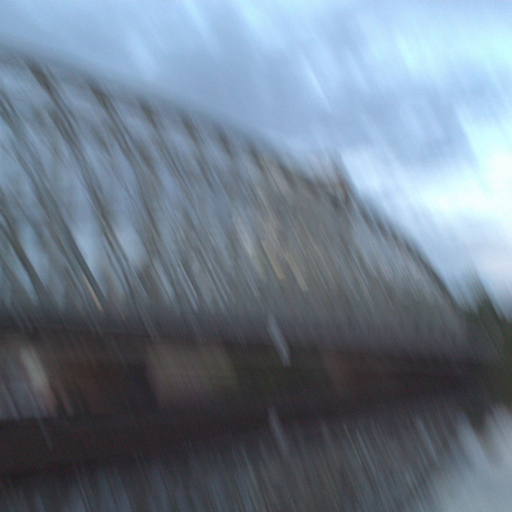
\includegraphics[width=.25\columnwidth,height=3cm]{images/bridge.png}}}
%     \qquad
%     \subfloat[Deblurred]{{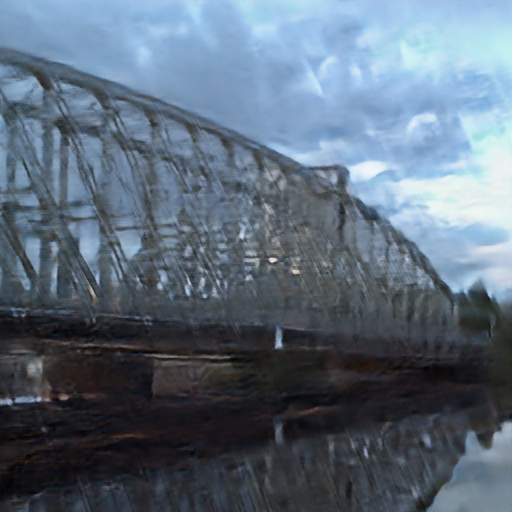
\includegraphics[width=.25\columnwidth,height=3cm]{images/bridge_dg.png}}}
% \end{figure}
% \begin{figure}[!H]
% \centering
% \begin{subfigure}{.5\textwidth}
%   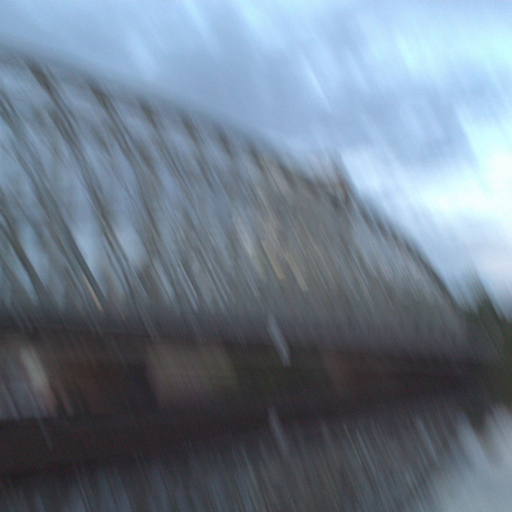
\includegraphics[width=.5\columnwidth,height=3cm]{images/bridge.png}
% \end{subfigure}%
% \hspace{\columnwidth}
% \begin{subfigure}{.5\textwidth}
%   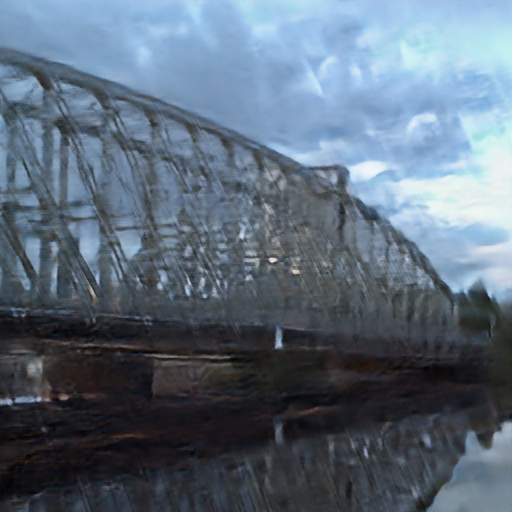
\includegraphics[width=.5\columnwidth,height=3cm]{images/bridge_dg.png}
% \end{subfigure}
% \begin{subfigure}{.5\textwidth}
%   \centering
%   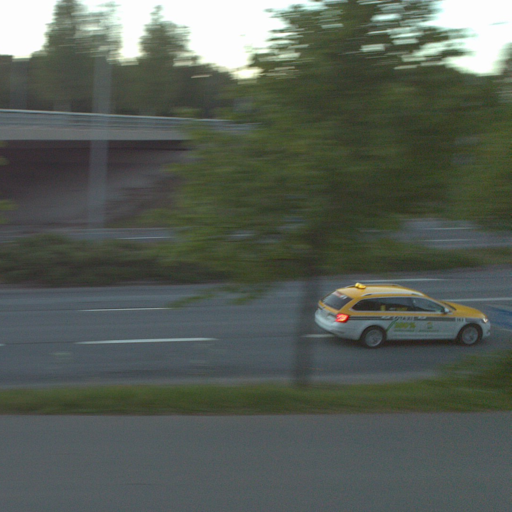
\includegraphics[width=.5\linewidth]{images/car.png}
% \end{subfigure}%
% \begin{subfigure}{.5\textwidth}
%   \centering
%   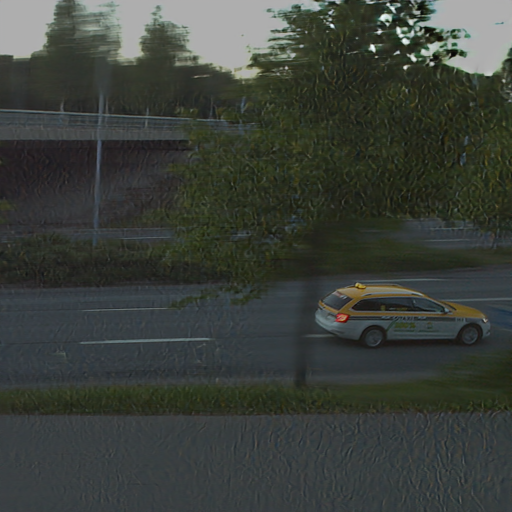
\includegraphics[width=.5\linewidth]{images/car_dg.png}\hfill
% \end{subfigure}
% \begin{subfigure}{.5\textwidth}
%   \centering
%   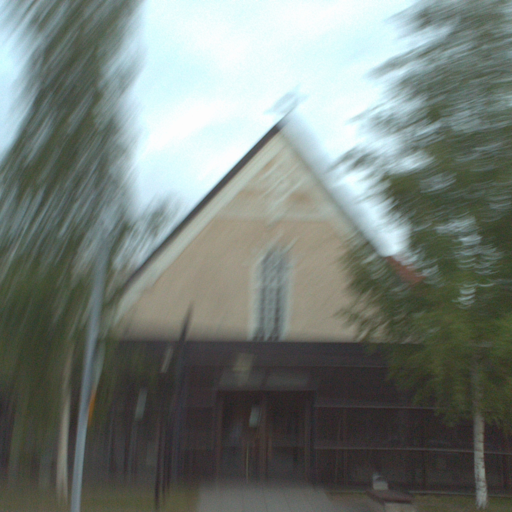
\includegraphics[width=.5\linewidth]{images/church.png}
% \end{subfigure}%
% \begin{subfigure}{.5\textwidth}
%   \centering
%   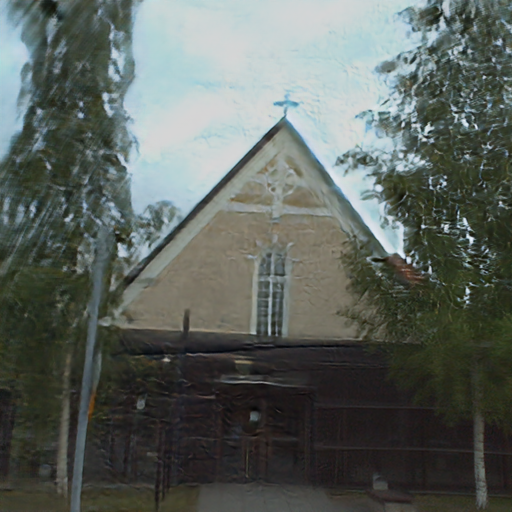
\includegraphics[width=.5\linewidth]{images/church_dg.png}\hfill
% \end{subfigure}
% \begin{subfigure}{.5\textwidth}
%   \centering
%   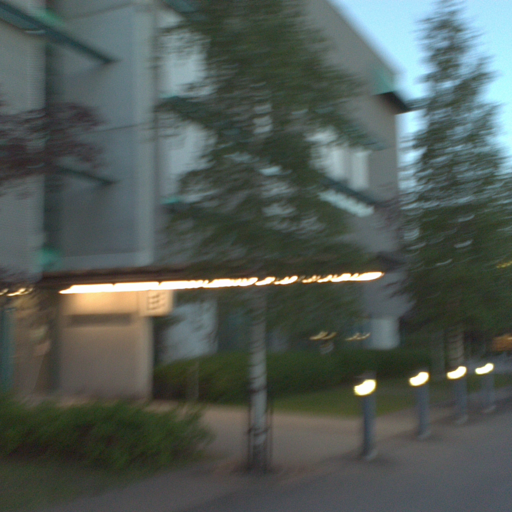
\includegraphics[width=.5\linewidth]{images/entrance.png}
% \end{subfigure}%
% \begin{subfigure}{.5\textwidth}
%   \centering
%   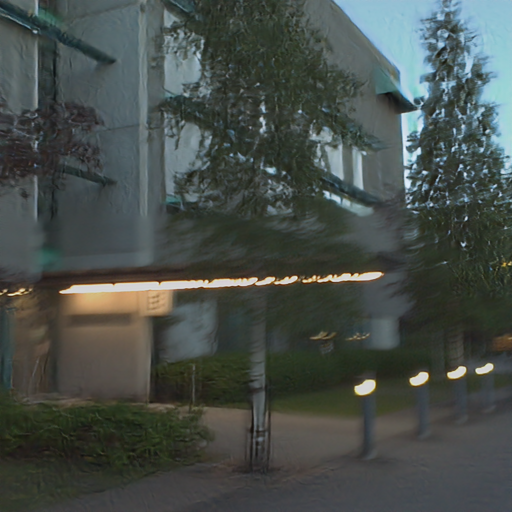
\includegraphics[width=.5\linewidth]{images/entrance_dg.png}\hfill
% \end{subfigure}
% \begin{subfigure}{.5\textwidth}
%   \centering
%   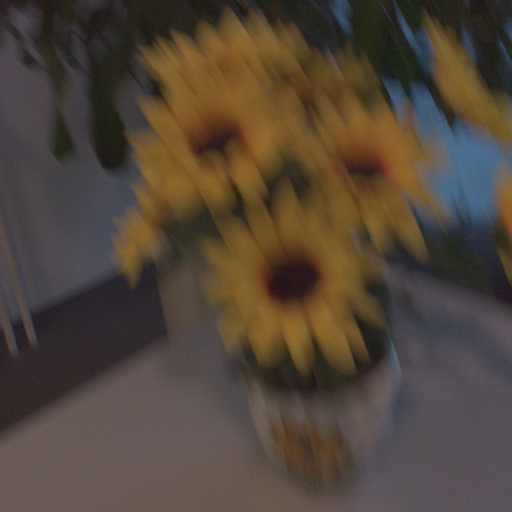
\includegraphics[width=.5\linewidth]{images/flower.png}
% \end{subfigure}%
% \begin{subfigure}{.5\textwidth}
%   \centering
%   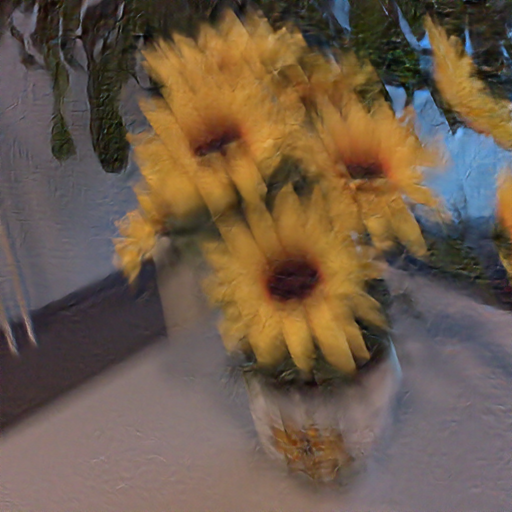
\includegraphics[width=.5\linewidth]{images/flower_dg.png}\hfill
% \end{subfigure}
% % \begin{subfigure}{.5\textwidth}
% %   \centering
% %   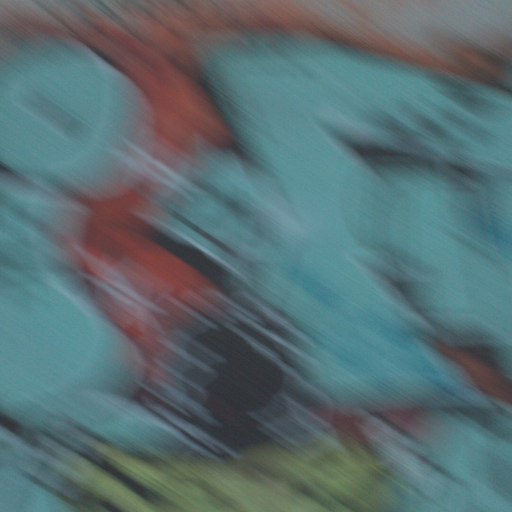
\includegraphics[width=.5\linewidth]{images/graffiti.png}
% % \end{subfigure}%
% % \begin{subfigure}{.5\textwidth}
% %   \centering
% %   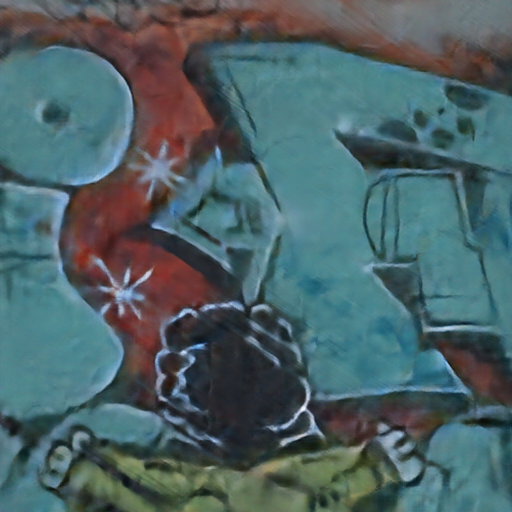
\includegraphics[width=.5\linewidth]{images/graffiti_dg.png}\hfill
% % \end{subfigure}
% % \begin{subfigure}{.5\textwidth}
% %   \centering
% %   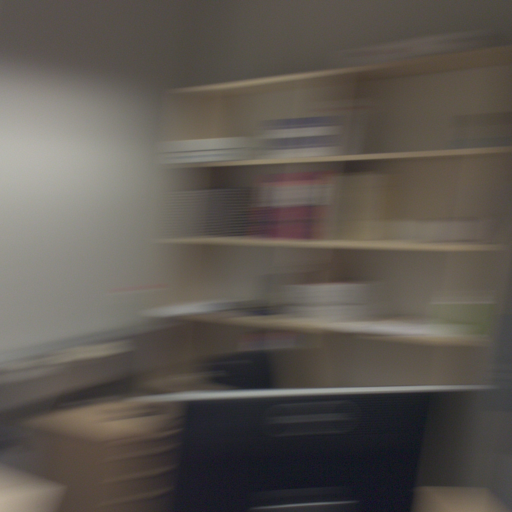
\includegraphics[width=.5\linewidth]{images/office.png}
% % \end{subfigure}%
% % \begin{subfigure}{.5\textwidth}
% %   \centering
% %   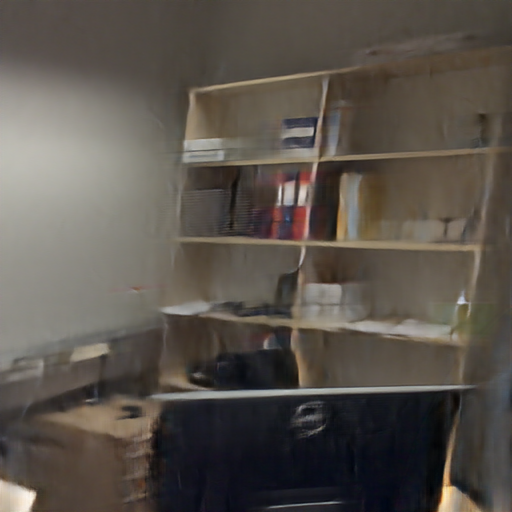
\includegraphics[width=.5\linewidth]{images/office_dg.png}\hfill
% % \end{subfigure}
% % \begin{subfigure}{.5\textwidth}
% %   \centering
% %   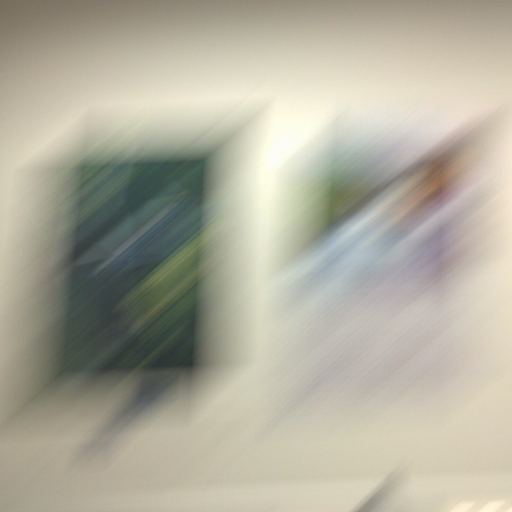
\includegraphics[width=.5\linewidth]{images/posters.png}
% % \end{subfigure}%
% % \begin{subfigure}{.5\textwidth}
% %   \centering
% %   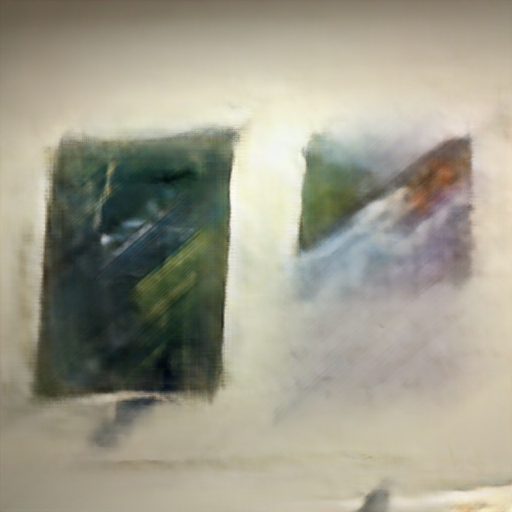
\includegraphics[width=.5\linewidth]{images/posters_dg.png}\hfill
% % \end{subfigure}
% % \begin{subfigure}{.5\textwidth}
% %   \centering
% %   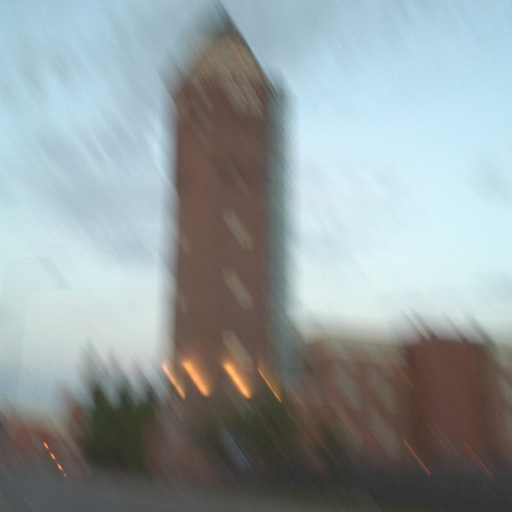
\includegraphics[width=.5\linewidth]{images/tower.png}
% % \end{subfigure}%
% % \begin{subfigure}{.5\textwidth}
% %   \centering
% %   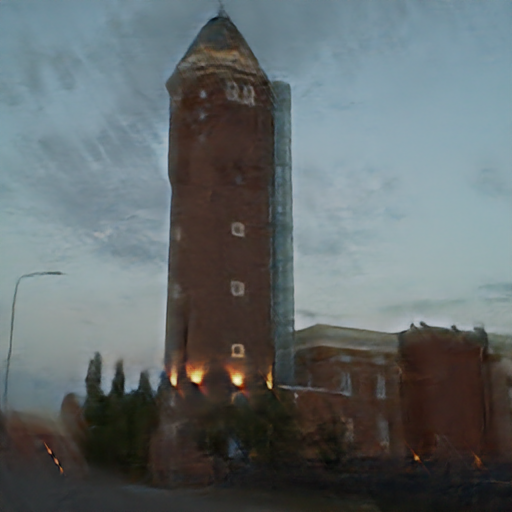
\includegraphics[width=.5\linewidth]{images/tower_dg.png}\hfill
% % \end{subfigure}
% \caption{Results replicated from the paper(blurred on left, deblurred on right)}
% \label{fig: ExampleBlurField}
% \end{figure}














\newpage
In Figure \ref{fig:real_pic}, few snapshots of real world are taken and deblurred.
\begin{figure}[h]
  \centering
  \begin{subfigure}{.5\columnwidth}
    \centering
    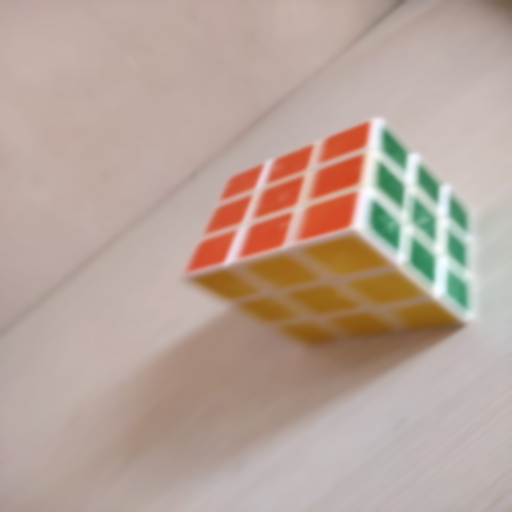
\includegraphics[width=\linewidth]{images/rubiks.png}
  \end{subfigure}%
  \hfill
  \begin{subfigure}{.5\columnwidth}
    \centering
    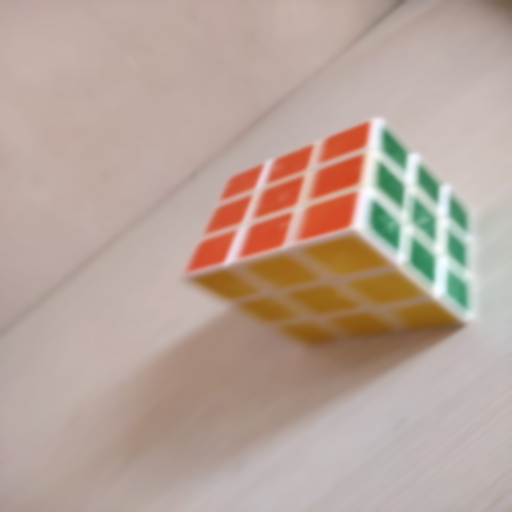
\includegraphics[width=\linewidth]{images/rubiks _db.png}
  \end{subfigure}%
  \hfill
\end{figure}
\vspace{-1cm}
\begin{figure}[h]
  \centering
  \begin{subfigure}{.5\columnwidth}
    \centering
    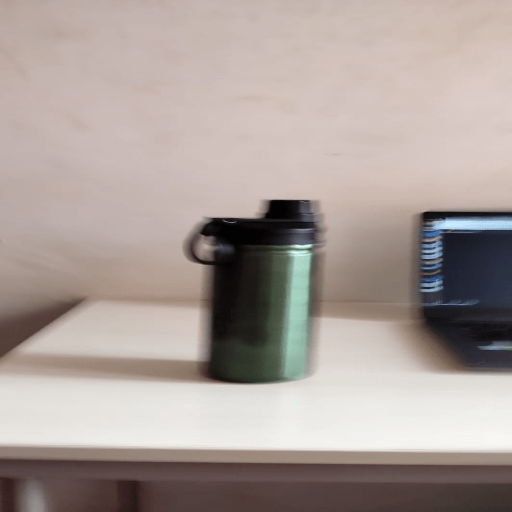
\includegraphics[width=\linewidth]{images/bottle.png}
  \end{subfigure}%
  \hfill
  \begin{subfigure}{.5\columnwidth}
    \centering
    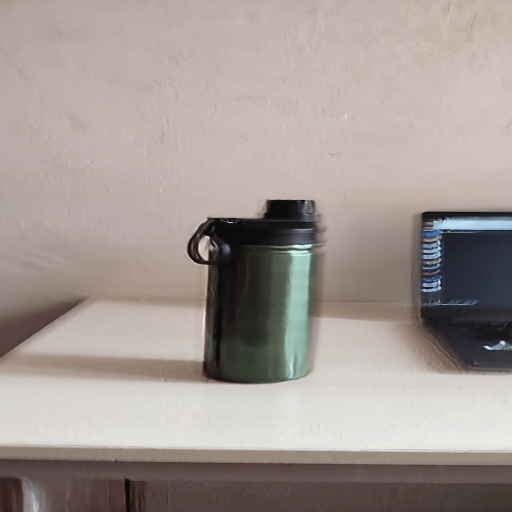
\includegraphics[width=\linewidth]{images/bottle_db.png}
  \end{subfigure}%
  \hfill
  \caption{Simulated Examples(blurred on left, deblurred on right)}
  \label{fig:real_pic}
\end{figure}
\section{MCG-GAN Network}

\subsection{Dataset for Model}
We used CIFAR-10 dataset for training our model. The CIFAR-10 dataset consists of 60000 32x32 colour images in 10 classes, with 6000 images per class. For testing the model, we picked 10 random images from each class of the dataset. So, the size of our training input is 100 32x32x3 images. The size of training input is small as the deep convolutional GAN takes lot of time to run for higher dataset sizes.

\subsection{Network Architecture}
Our GAN\footnote[1]{\href{https://drive.google.com/drive/folders/1XLaAKyKIWfiOekj9VXCfOz7ow2UZIJ4v?usp=sharing}{Drive folder link containing training model}} includes 1 generator and 1 discriminator. The generator takes an input of dimension noise-dim(noises to make image look blurry), and through multiple sets of dense layers followed by LeakyReLu activations, it outputs a flat version of the image(unblurred version). 
\\
We added noise to normal images instead of taking blurred images we created for now to test the validity of model. As the model is performing well now, the generator of final DCG-GAN will take blurred image and motion blur data and work to return an image which can fool the discriminator to believe it’s a real image. Which in our case means, creating a deblurred image from given blurred image. 
\\
This model starts with a small image, which is slowly scaled up with Conv2DTranspose layers. Growing GAN images is an incredible technique developed by NVIDIA, and the generator architecture above mimics a greatly simplified version of it. For the final layer we are using tanh activation function as it gives better results and normalizes our image.
\\
The optimizer we use is also very important, in our model we decided to use Adam optimizer as Adam combines the best properties of the AdaGrad and RMSProp algorithms to provide an optimization algorithm that can handle sparse gradients on noisy problems.

\begin{figure}[h]
    \centering
    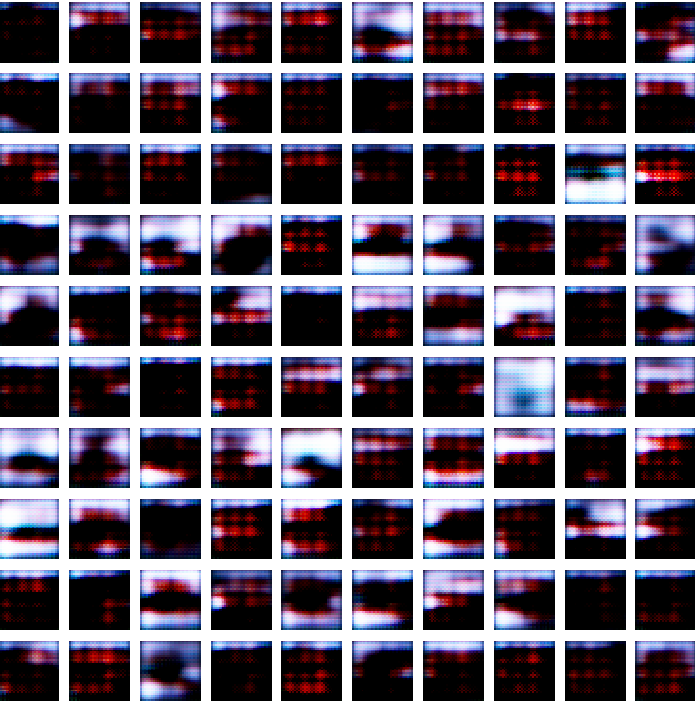
\includegraphics[width=1\columnwidth,height=6cm]{images/Before.png}
    \caption{ Before training}
    \label{fig: before_training}
\end{figure}

In Figure \ref{fig: before_training} we have 100 images after adding noises. Which in our case means before training and after training these images for 320 epochs we got Figure \ref{fig: after_training}.

\begin{figure}[h]
    \centering
    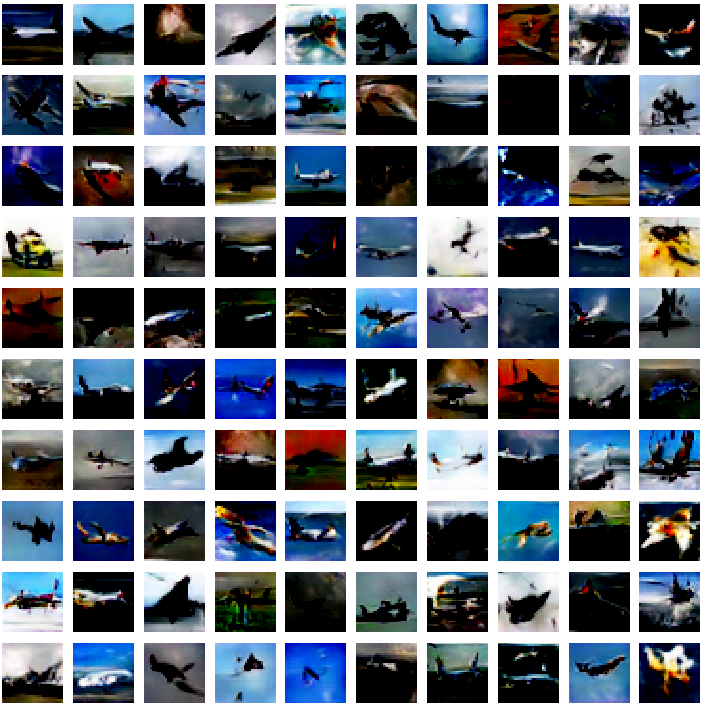
\includegraphics[width=1\columnwidth,height=6cm]{images/After.png}
    \caption{ After training}
    \label{fig: after_training}
\end{figure}
%%%%%%%%% REFERENCES
{\small
\bibliographystyle{ieee_fullname}
\bibliography{egbib}
}
\end{document}
